\chapter{Introduction}
\label{chapter:Introduction}
Modern software system are heterogeneous in terms of \glspl{Language} and \glspl{Technology} used for programming and inter process communication, which is a challenge for program comprehension.
Support of \glspl{Traceability} can provide help to overcome this challenge by bringing out related components of a software system.
 


\section{Motivational Example}
Common tasks in software development are implementation of serialization and persistence of domain models.
For instance, consider a simple web service which serves data via \gls{HTTP} as \gls{XML} and stores it in a relational database.
We call this an \gls{O/R/X-Mapping} scenario.
Given such a system, the same conceptual data, i.e. the domain model, is transported through application tiers in different forms, that is, the same data is represented by various manifestations at a time.
Each manifestation involves another software language and technology.
\begin{figure}[h!]
\begin{center}
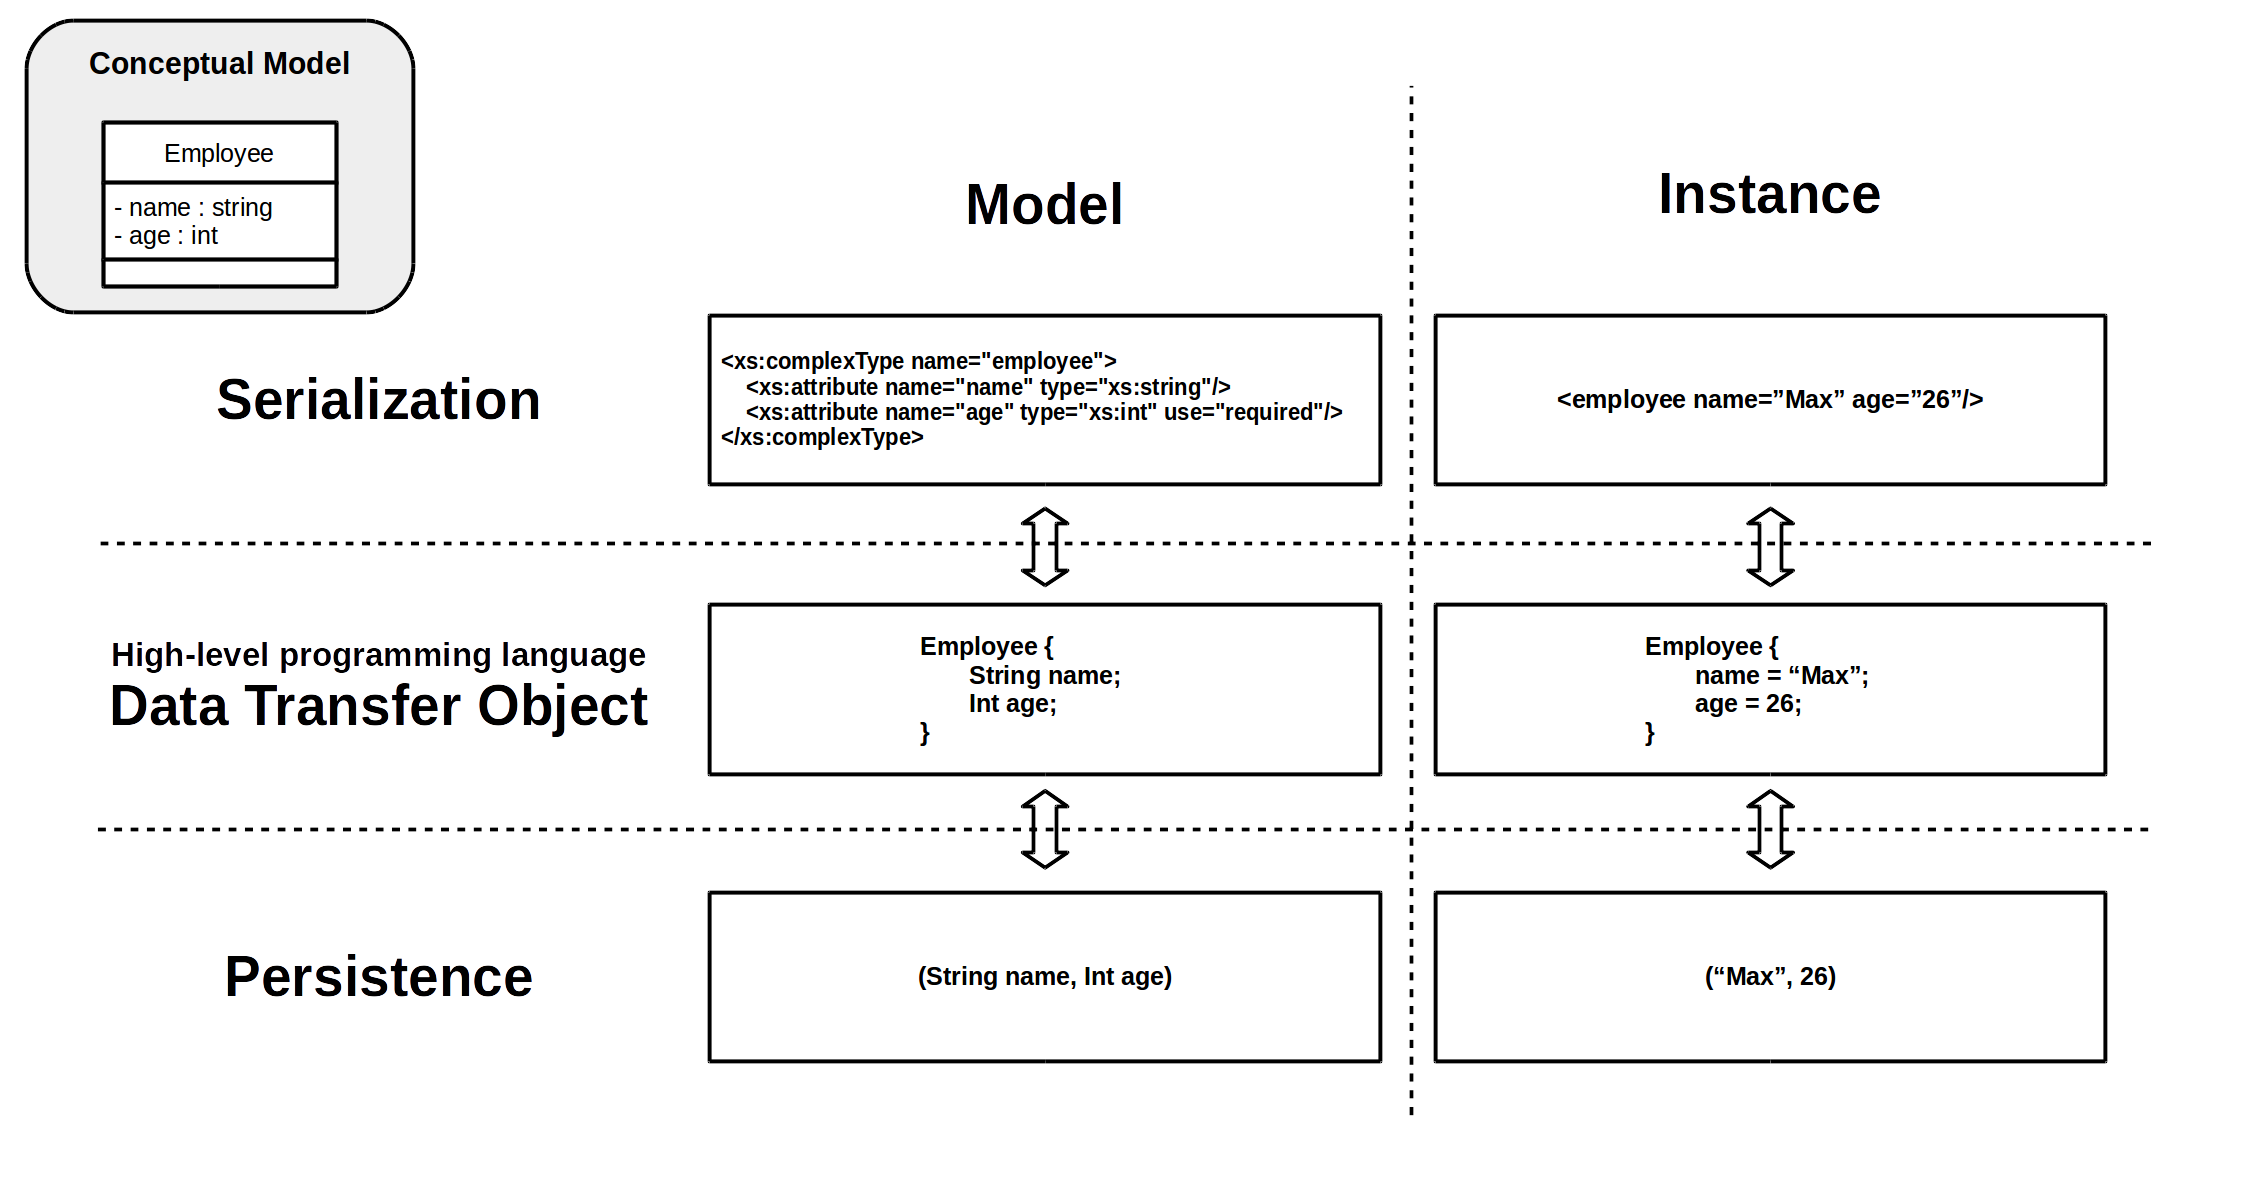
\includegraphics[width=.9\textwidth]{images/ORX.png}
\end{center}
\caption{O/R/X-Mapping Manifestations}
\label{figure:ORXManifestations}
\end{figure}
Figure \ref{figure:ORXManifestations} opposes model- to instance-level syntaxes of different manifestations for a conceptual model for employees in an \gls{O/R/X-Mapping} scenario.
One employee only has a \textit{name} and an \textit{age} attribute.
Persistence is presented in tuple notation, data transfer objects of an application tier are represented with a fictional high level programming language object notation and serialization is exemplified with \gls{XML} and \gls{XSD} syntax.

Although figure \ref{figure:ORXManifestations} shows a fictionalized example, one can observe structural similarities among the different model and instance representation syntaxes.
Such similarities also occur in real-world software engineering through use of conventions which may be predefined in technologies for \gls{O/R/X-Mapping}.
\begin{figure}[h!]
\begin{center}
\begin{minipage}{.49\textwidth}
\begin{lstlisting}[language=Java,numbers=none]
@XmlRootElement(name="employee")
@XmlAccessorType(XmlAccessType.FIELD)
public class Employee {

	@XmlAttribute
	private int id;
	
	@XmlAttribute
	private String name;
	
	@XmlAttribute
	private int age;
	
	@XmlAttribute
	private double salary;
	
	private Department department;
	
	private Department managedDepartment;
	
}
\end{lstlisting}
\end{minipage}
\hspace*{\fill}
\begin{minipage}{.49\textwidth}
\begin{lstlisting}[language=XML,numbers=none]
<xs:complexType name="employee">
 <xs:attribute name="id" type="xs:int" use="required"/>

 <xs:attribute name="name" type="xs:string"/>

 <xs:attribute name="age" type="xs:int" use="required"/>

 <xs:attribute name="salary" type="xs:double" use="required"/>
 
 <xs:sequence>
 
   <xs:element ref="department" minOccurs="0"/>
 
   <xs:element name="managedDepartment" type="department" minOccurs="0"/>
 
 </xs:sequence>
</xs:complexType>
\end{lstlisting}
\end{minipage}
\begin{minipage}{\textwidth}
\begin{lstlisting}[language=XML,numbers=none]
<employee name="Max" age="26" salary="55000.0"/>
\end{lstlisting}
\end{minipage}
\end{center}
\caption{JAXB XML/XSD Mapping}
\label{figure:JAXBMapping}
\end{figure}
Figure \ref{figure:JAXBMapping} displays an annotated \gls{Java} class and \gls{XML}/\gls{XSD} output generated by \gls{JAXB}.
Except for the root element all names for attributes and elements are taken from the \gls{Java} class.
Moreover, the \gls{XSD} complex type and the \gls{Java} class share a similar nested structure.
Links through similarity can be found within the model-level \glspl{Representation} (\gls{Java}-\gls{XSD}) and between model- and instance-level \glspl{Manifestation} (\gls{Java}-\gls{XML} and \gls{XSD}-\gls{XML}), for instance:
\begin{itemize}
\item
\texttt{public class Employee \{...\}} is linked with \texttt{<xs:complextType name="employee">...</xs:complexType>}
and \texttt{<employee .../>}, the latter two are also linked with each other

\item
\texttt{private String name;} is linked with \texttt{<xs:attribute name="name" type="xs:string"/>} and \texttt{name="Max"}, the latter two are also linked with each other
\end{itemize}


\section{Objectives}
\label{section:Objectives}

The aim of this thesis is to provide automated recovery of such similarities as semantic links.
Recovered links are inserted into \textit{\glspl{Megamodel}} \cite{DBLP:conf/sattose/BaggeZ14} \cite{DBLP:journals/entcs/FavreN05} for \textit{\glspl{LinguisticArchitecture}} \cite{DBLP:conf/models/FavreLV12} \cite{DBLP:conf/ecmdafa/LammelV14} \cite{HeinzLV17}.
\Glspl{Megamodel} are models providing a high level of abstraction with other models as modeling elements, e.g. a \gls{Megamodel} may describe the dependencies between \glspl{Metamodel}, models and instances.
\Glspl{LinguisticArchitecture} intend to describe software systems from a language centric point of view.
They model knowledge about software systems in terms of \glspl{Language}, \glspl{Artifact}, \glspl{Technology}, etc.
Such entities are interrelated with relationships derived from common software engineering and theoretical computer science vocabulary providing special semantics, e.g. \textit{defines}, \textit{isA}, \textit{instanceOf}, \textit{represents}, \textit{implements}, \textit{realizationOf}, \textit{elementOf}, \textit{subsetOf}.

\Glspl{LinguisticArchitecture} are related to \glspl{ERModel} and \glspl{Ontology}.
Recovering semantic links as described above is related to the concept of \textit{\gls{Traceability}} and an application of \textit{\gls{TraceabilityRecovery}} \cite{DBLP:books/daglib/p/GotelCHZEGDAMM12} (see §\ref{section:Traceability}).
In context of \gls{Traceability}, semantic links may be called \textit{\glspl{TraceLink}}, however, both establish a relation between two entities denoting a certain meaning.

\Glspl{TraceLink} among software \glspl{Artifact} denoting that one \gls{Artifact} encodes the same information as the other are called \textit{\gls{Correspondence}} links and denoted \textit{correspondsTo} (see §\ref{subsection:Correspondence}).
\Glspl{TraceLink} between two \glspl{Artifact} denoting that one defines the other, in the sense of a \gls{Metamodel} defining a model, are called \textit{\gls{Conformance}} links and denoted \textit{conformsTo} (see §\ref{subsection:Conformance}).
The main objective is to recover such \glspl{TraceLink} among well-formed, possibly partial, source code \glspl{Artifact}.
We call well-formed partial source code \glspl{Artifact} \textit{\glspl{Fragment}} (see §\ref{subsection:Fragments}).
 

\section{Approach}
\label{section:Approach}
Our approach for recovering \glspl{TraceLink} utilizes \textit{\gls{StaticProgramAnalysis}}.
We use it in the broad sense that we construct specialized \glspl{AST} for further analysis.
Usually \gls{StaticProgramAnalysis} is used with the purpose of formal verification or measurement of software engineering related properties of source code, e.g. cohesion and coupling metrics.
We use \gls{StaticProgramAnalysis} to semantically link code \glspl{Fragment} and uncover knowledge of the analyzed \glspl{Artifact}.
In that respect, our approach is related to computing software metrics.

\begin{figure}[h!]
\begin{center}
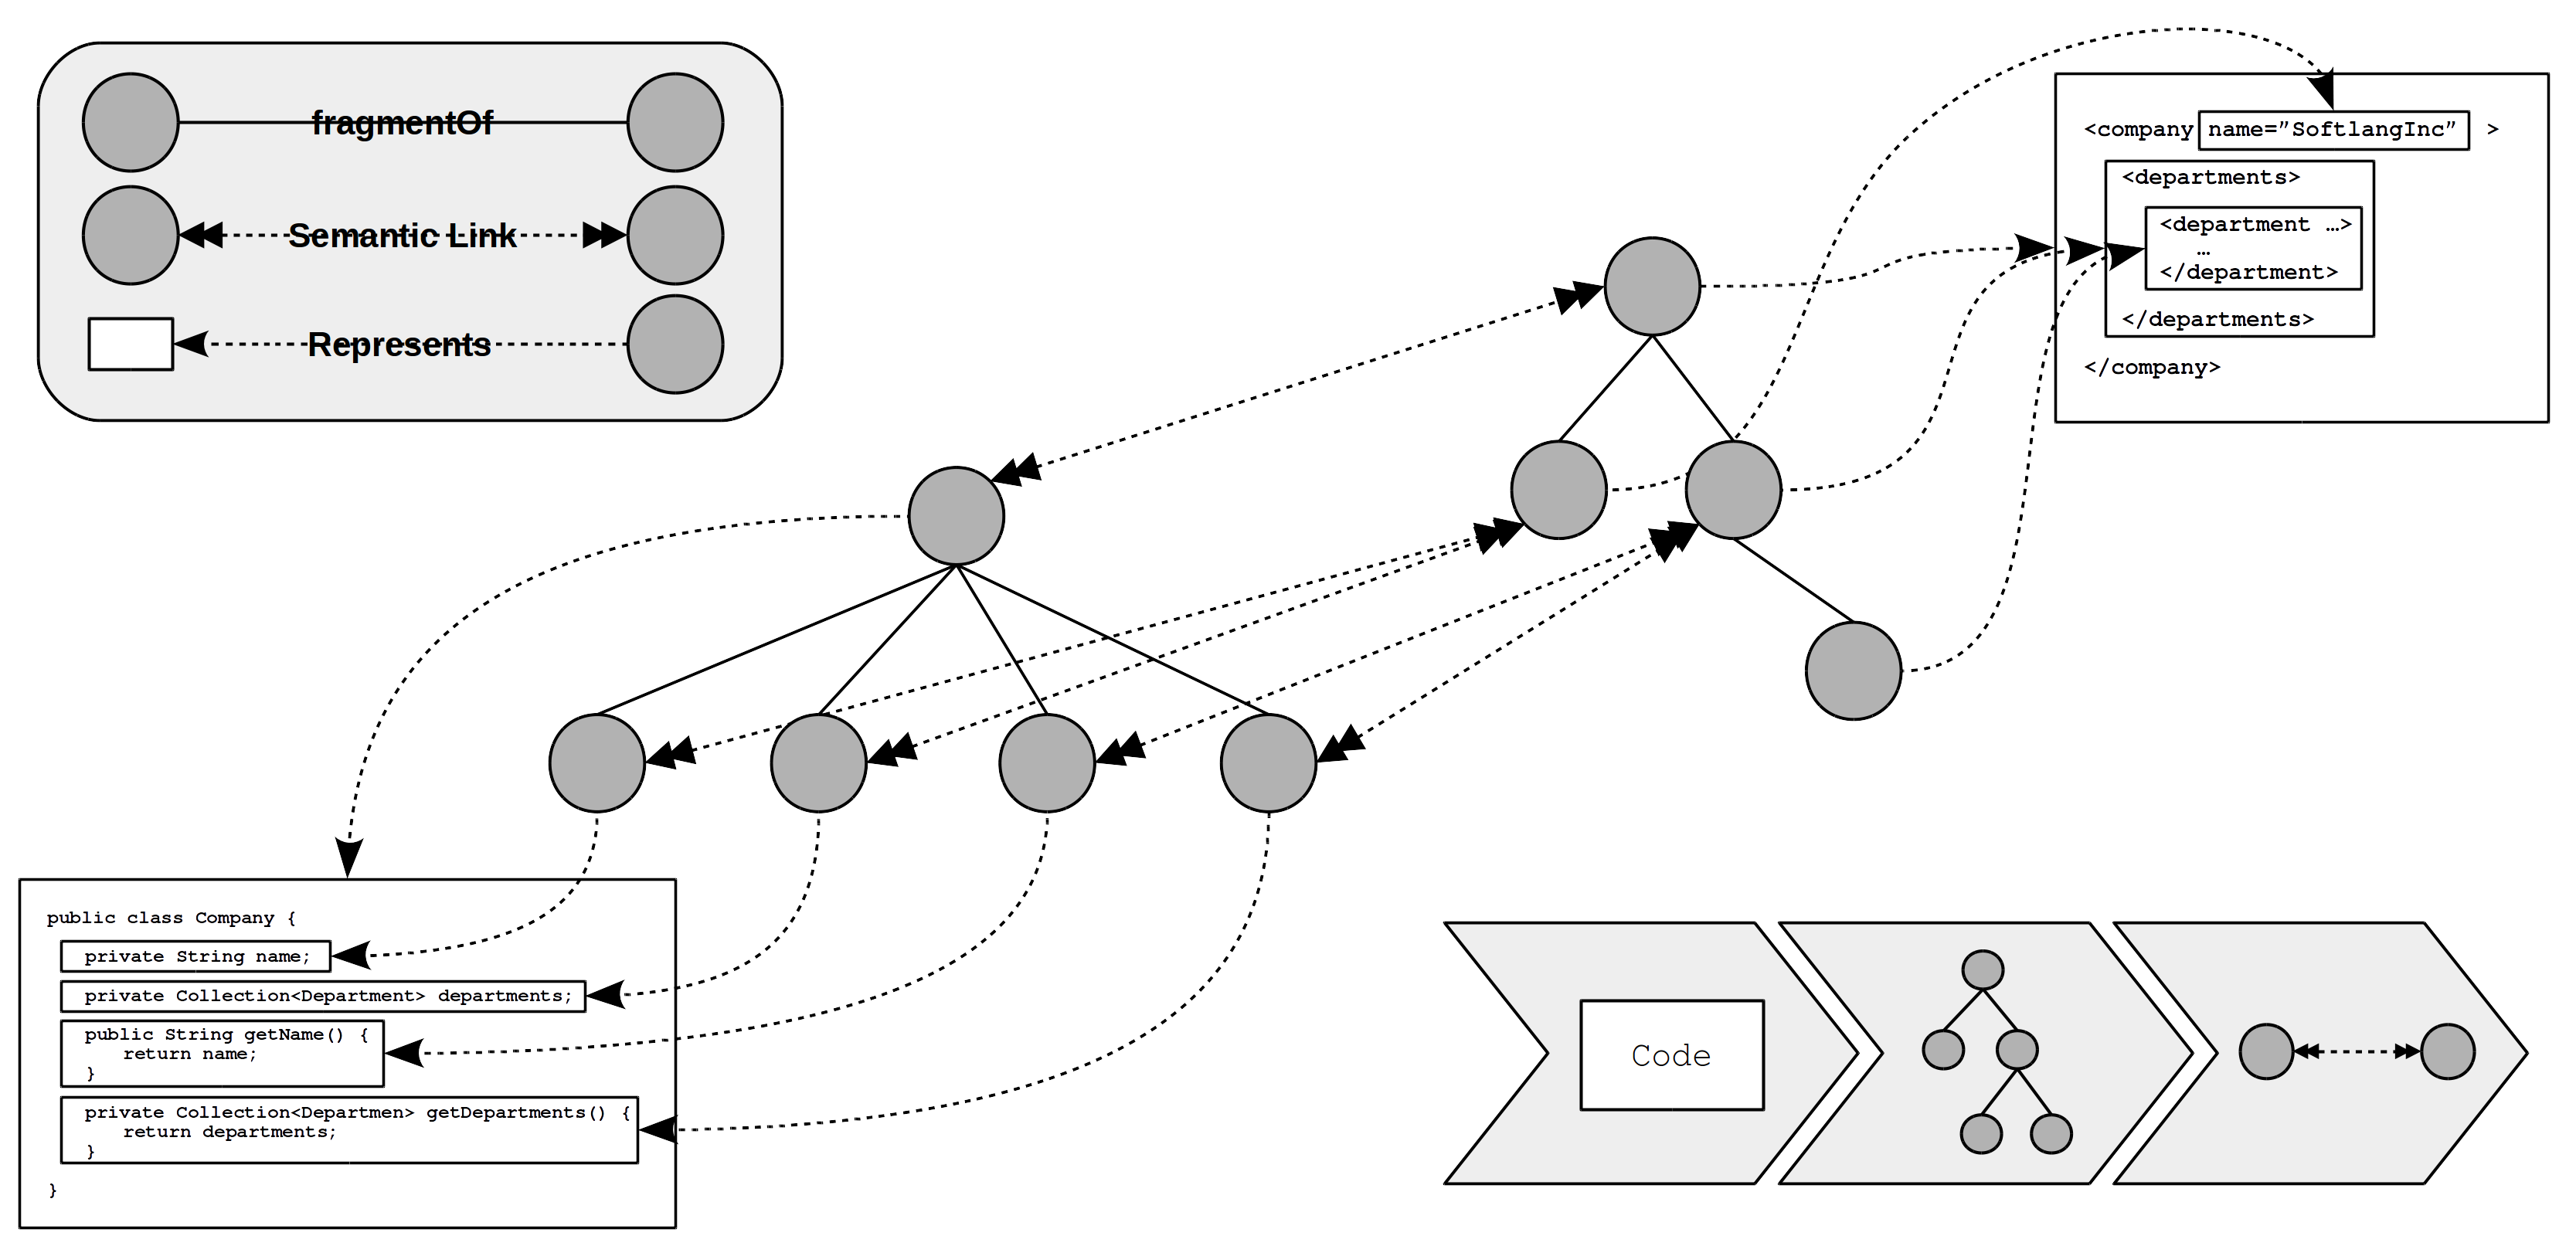
\includegraphics[width=\textwidth]{images/RecoveryExample.png}
\end{center}
\caption{Recovery Approach}
\label{figure:RecoveryApproach}
\end{figure}
Figure \ref{figure:RecoveryApproach} shows a schematic illustration of our recovery approach.
It can be summarized with the following three steps:
\begin{enumerate}
\item
we create two \glspl{ParseTree} for both inputs respectively
\item
\glspl{ParseTree} are transformed to specialized \glspl{AST};
such \glspl{AST} are not intended to be used for compilation, instead each node represents a part of code which may be linked during further analysis;
a child node represents a piece of code which is properly embedded the code represented by its parent
\item
we apply a comparative analysis to both \glspl{AST};
while traversing through both trees we check whether each pair of nodes is a \gls{TraceLink}
\end{enumerate}

\section{Contributions \& Non-Contributions}
\label{section:ContributionsAndNonContributions}
This section lists critical contributions and non-contributions of this thesis:

\begin{contributions}

\item
We contribute a \gls{Java} based \gls{API} for recovering \glspl{TraceLink} among \glspl{Artifact} and their constituent \glspl{Fragment}, providing utilities for \gls{StaticProgramAnalysis} as described in §\ref{section:Approach} (see §\ref{chapter:Design}).

\item
We contribute an implementation for \gls{Correspondence} and \gls{Conformance} link recovery among \gls{JAXB} and \gls{Hibernate} \glspl{Artifact} utilizing the created \gls{API} and axioms for linguistic architectures (see §\ref{chapter:Implementation} and §\ref{section:AxiomsOfLinguisticArchitectures} respectively).

\item
We contribute a small case-study applying the implemented recovery system to a minimal \gls{O/R/X-Mapping} program (see §\ref{chapter:MiniCaseStudy}).

\end{contributions}

\begin{noncontributions}

\item
We do not contribute to the axiomatization of linguistic architectures as described in \cite{DBLP:conf/ecmdafa/LammelV14}, \cite{DBLP:journals/entcs/FavreN05}, \cite{DBLP:conf/sle/Lammel16} and \cite{HeinzLV17}.

\end{noncontributions}

\section{Road-Map}
§\ref{chapter:Background} provides the necessary theoretical and practical background for this thesis.
§\ref{chapter:RelatedWork} provides a summary on related work and positions this thesis among these works.
§\ref{chapter:Design} provides a high level design description for the system developed for this thesis.
§\ref{chapter:Implementation} provides a more detailed description of the implementation for crucial components of the developed system.
§\ref{chapter:MiniCaseStudy} provides a mini case-study evaluating the developed system.
§\ref{chapter:Conclusion} concludes the thesis.
